\begin{summary}
\section{Contexte}
Ce laboratoire a servi a implémenter des patternes orienté-objet,
servant à découpler différents modules. Ces patternes permettent de
réaliser du code plus portable, moins dépendant du Hardware de base.
Le module \emph{XF (Execution Framework)} est utilisé ici pour créer des
machines d'états et aidé a réaliser un code pseudo-parallèle.
\end{summary} \newpage

\section{Objectifs}
L'objectif de ce laboratoire est de réaliser un loggeur de bouton, qui affiche si le bouton
a été appuyé rapidement, ou laissé enfoncé.
Chaque \emph{couche} de ce projet doit être découplée au mieux de la \emph{couche} en dessous,
pour rendre le projet portable et adaptatif. Les \emph{couches} sont les suivantes :
Application, avec la \emph{Factory} et le \emph{ButtonEventsLogger}. Middleware, avec
le \emph{ButtonEventsHandler} et les \emph{ButtonStateSM}. Et au fond, la Board Layer avec
le \emph{ButtonsController}.
Le module \emph{XF} développé aux précédents labos a été utilisé pour
permettre un programme pseudo-parallèle.
\begin{figure}[H]
    \centering
    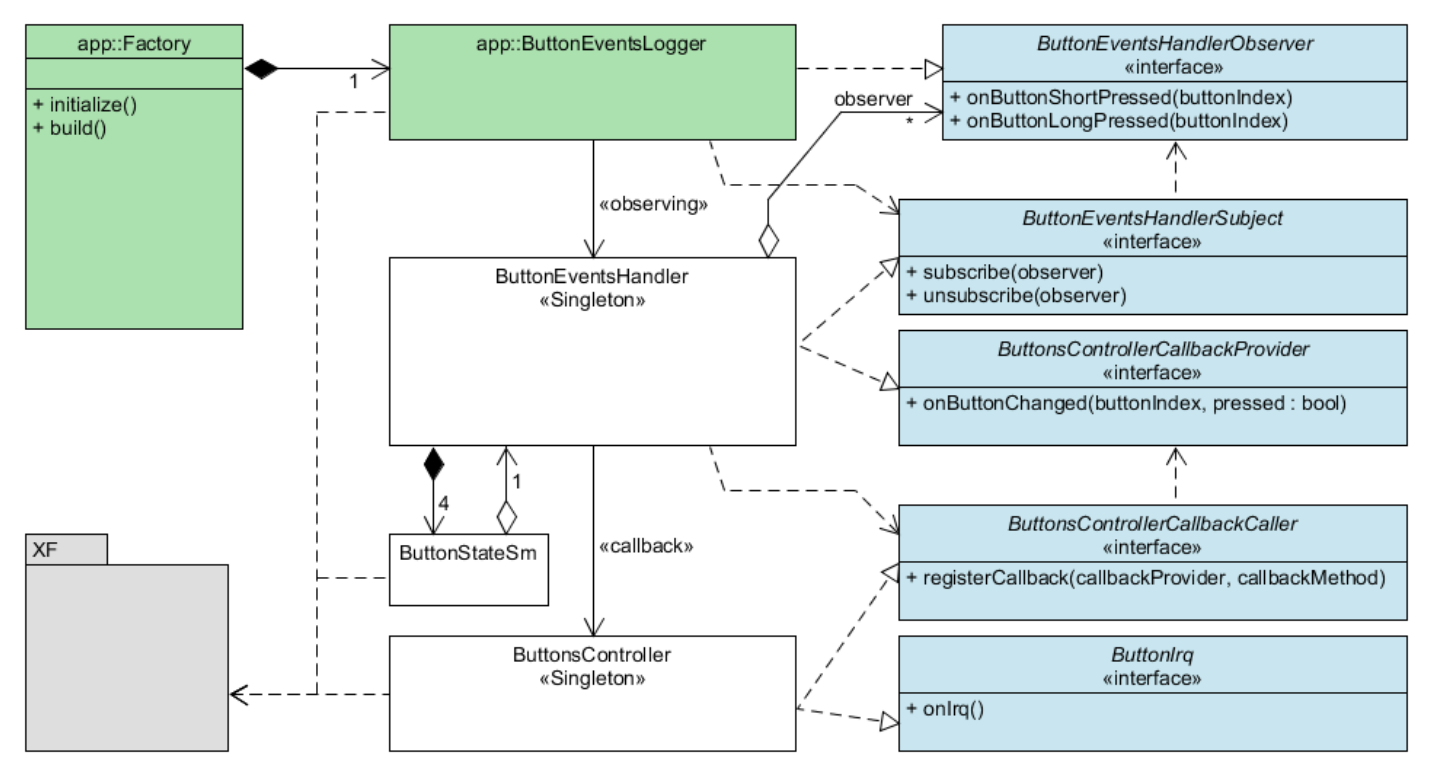
\includegraphics[width=1\textwidth]{Images/buttons/full_uml.PNG}
    \caption[Full UML]{Diagramme de classe complet du contrôleur
    (provenant du \emph{Guide ButtonsController}\footnotemark)}
\end{figure}
\footnotetext{\cite{lab_guide}}
